%! alt Two triangles share side AB = 8 and the 60 degree angle at A. The third vertex lies on the same ray from A, at C with AC = 3 or at C' with AC' = 5. Both points are at distance 7 from B, on a dashed arc centred at B.
%! after_paragraph 1
%! scale 2/5
% The shared preamble of every Cevian figure. pipeline/figures turns these colours into theme-aware paint,
% and refuses any other colour, so draw only with them:
%   figink (lines and labels), figaux (construction lines), figaccent (the object the argument turns on),
%   figtint and figaccenttint (light fills).
\documentclass[border=1.5pt]{standalone}
\usepackage{tkz-euclide}
\definecolor{figink}{RGB}{0,0,0}
\definecolor{figaux}{RGB}{85,85,85}
\definecolor{figaccent}{RGB}{192,57,43}
\definecolor{figtint}{RGB}{221,221,221}
\definecolor{figaccenttint}{RGB}{245,213,208}
% tkz-euclide's defaults draw circles, compasses and marks in 50% grey and fill points with a tint.
\makeatletter
\def\tkz@otherlinecolor{figink}
\def\tkz@euc@circlecolor{figink}
\def\tkz@euc@compasscolor{figink}
\def\tkz@euc@mkcolor{figink}
\def\tkz@mk@fill{figink}
\def\tkz@euc@pointfillcolor{figink}
\makeatother
\tkzSetUpLine[color=figink,line width=.7pt]
\tkzSetUpArc[color=figink,line width=.7pt]
\tkzSetUpCompass[color=figink,line width=.5pt]
\tkzSetUpPoint[color=figink,fill=figink,size=3.1pt]
\tikzset{
  every picture/.style={line cap=round,line join=round,color=figink},
  circle style/.append style={color=figink,line width=.7pt},
  aux/.style={color=figaux,line width=.45pt,dash pattern=on 2.6pt off 2pt},
  key/.style={color=figaccent,line width=1pt},
  mk/.style={color=figink,line width=.5pt},
  lbl/.style={color=figink,inner sep=2.2pt},
  len/.style={color=figink,inner sep=1.5pt,font=\small},
}

\begin{document}
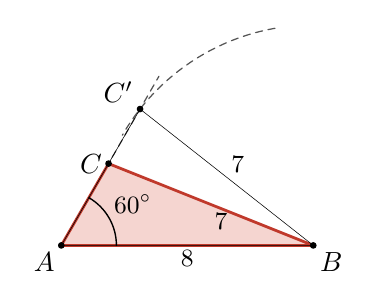
\begin{tikzpicture}
\tkzDefPoint(0.0,0.0){A} %! A = (0, 0)
\tkzDefPoint(3.2000000,0.0){B} %! B = (8, 0)
\tkzDefPoint(0.60000000,1.0392305){C} %! C = polar(A, 3, 60)
\tkzDefPoint(1.0000000,1.7320508){Cp} %! Cp = polar(A, 5, 60)
\tkzDefPoint(2.7137851,2.7574617){X} %! X = polar(B, 7, 100)
\tkzDefPoint(0.77512887,1.4000000){Y} %! Y = polar(B, 7, 150)
\tkzDefPoint(1.2400000,2.1477430){Z} %! Z = polar(A, 6.2, 60)
%! fact angle(B, A, C) == 60
%! fact dist(B, C) == 7
%! fact dist(B, Cp) == 7
%! fact dist(A, C) == 3
%! fact dist(A, Cp) == 5
%! fact collinear(Cp, A, C)
\tkzFillPolygon[color=figaccenttint](A,B,C)
\tkzDrawArc[aux](B,X)(Y)
\tkzDrawSegment[aux](A,Z)
\tkzDrawPolygon[key](A,B,C)
\tkzDrawPolygon(A,B,Cp)
\tkzMarkAngle[size=.7,arc=l,mark=none,mk](B,A,C)
\tkzLabelAngle[pos=1.05,font=\small](B,A,C){$60^\circ$}
\tkzDrawPoints(A,B,C,Cp)
\tkzLabelPoint[below left,lbl](A){$A$}
\tkzLabelPoint[below right,lbl](B){$B$}
\tkzLabelPoint[left,lbl](C){$C$}
\tkzLabelPoint[above left,lbl](Cp){$C'$}
\tkzLabelSegment[below,len](A,B){$8$}
\tkzLabelSegment[below,pos=.45,len](B,C){$7$}
\tkzLabelSegment[above right,len](B,Cp){$7$}
\end{tikzpicture}
\end{document}
